\documentclass{article}
\usepackage{amsmath}
\usepackage{listings}
\usepackage{moreverb}
\usepackage[margin=1in]{geometry}
\usepackage{graphicx}
\usepackage{dsfont}
\title{STA 360: Practice Question}
\author{Michael Lin}

\begin{document}
\maketitle

Suppose $X_{1:n}$ have negative binomial distribution with pmf:
$$ p(x|\theta) = \binom{x-1}{4} \theta^5 (1-\theta)^{x-5} $$
and suppose $\theta$ has a Beta(4,6) prior distribution. Find the posterior distribution of $\theta$ given $X_{1:n}$.

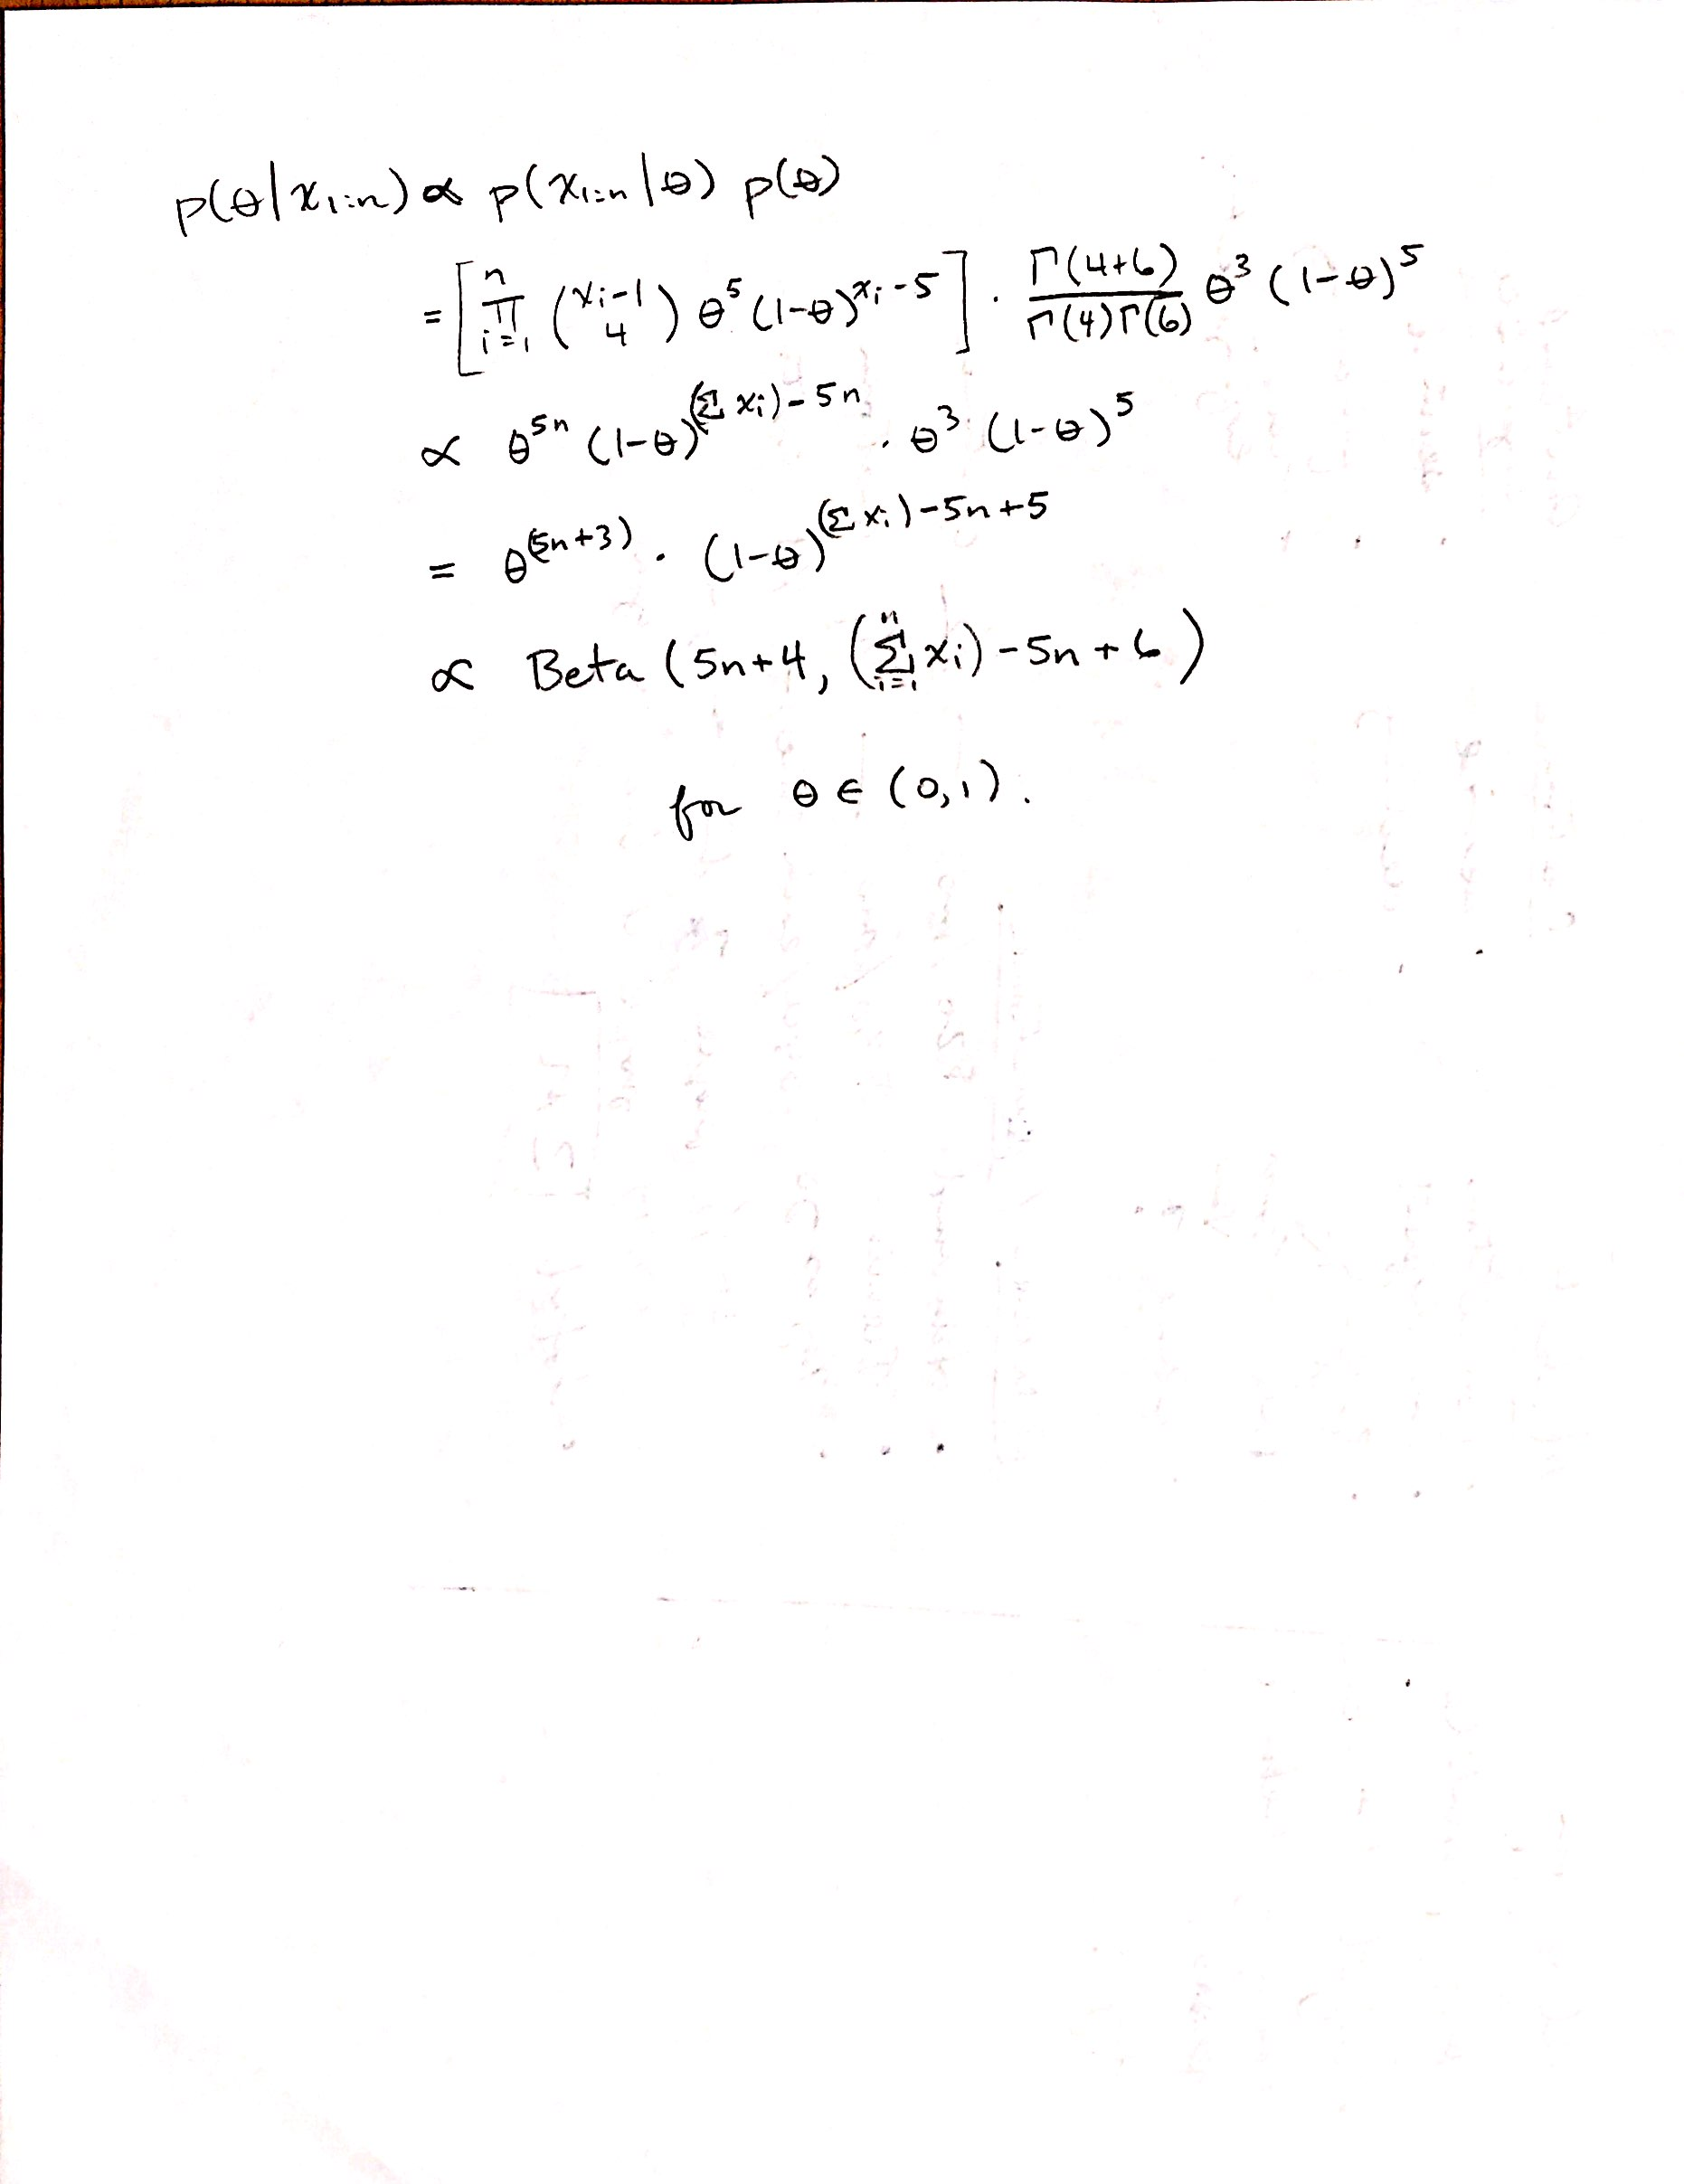
\includegraphics[scale = 0.25]{practice.jpg}

\end{document}